\documentclass{article}

\usepackage[spanish]{babel}
\usepackage[numbers,sort&compress]{natbib}
\usepackage[T1]{fontenc}
\usepackage[ansinew]{inputenc}
\usepackage{graphicx}
\usepackage{url}
\usepackage{caption}
\usepackage{subcaption}
\usepackage{float}

\title { Teor\'ia de Colas}
\author{Oscar Qui\~nonez}

\begin{document}

\maketitle
 
\section{Objetivo}\label{met}

En la presente simulaci\'on, se intenta reproducir la llamada``Teor\'ia de colas'' utilizando un archivo que contiene n\'umeros primos previamente generados.

\section{Metodolog\'ia}\label{met}

Esta simulaci\'on fue realizada usando como herrameinta el programa Python 3, donde se examin\'o el archivo que conten\'ia miles de n\'umeros primos y que la ser ejecutado, se var\'io el uso de los n\'ucleos que tiene el procesador instalado en el ordenador. Para realizar esta simulaci\'on fue necesario el uso de las instrucciones \cite{satuelisa} de la tarea 3, donde se menciona que los n\'umeros primos deben de tener por lo menos 8 d\'igitos, adem\'as del apoyo en el repositorio  \citet{baz} como base de l c\'odigo utilizado.

\section{Resultados y Discusi\'on}\label{res}

Al realizar la simulaci\'on en Python 3 se obtuvieron una serie de datos para 1000, 2000, 3000 y hasta 4000 n\'umeros del archivo auxiliar, a partir de los cuales se pudieron generar dos tipos de gr\'aficas, una con respecto al uso de los n\'ucleos contra la cantidad de datos y otra de n\'ucleos contra tiempo. Se pueden observar estas gr\'aficas a continuaci\'on.

\begin{figure}[H]
       \centering
       \begin{subfigure}[b]{0.45\linewidth}
           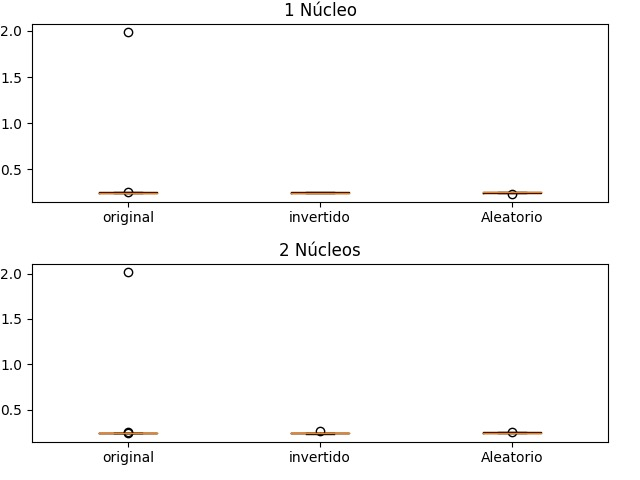
\includegraphics[width=\linewidth]{tareatresparamil.jpeg}
           \caption{Gr\'afica para mil n\'umeros usando dos procesadores.}
           \label{fig:westminster_lateral}
        \end{subfigure}
        \begin{subfigure}[b]{0.45\linewidth}
            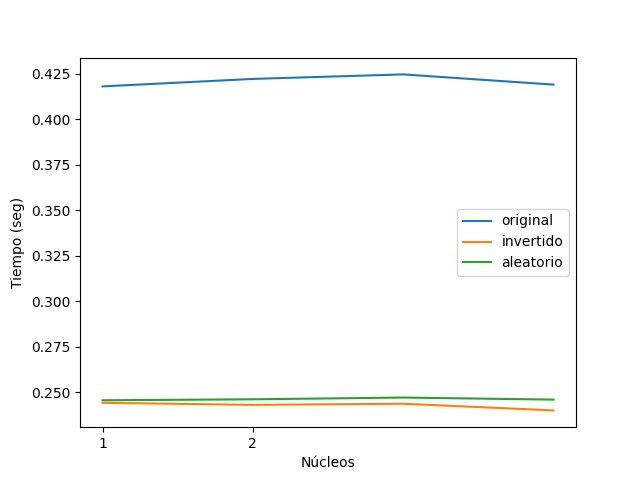
\includegraphics[width=\linewidth]{tareatresparamilgrafica.jpeg}
            \caption{Gr\'afica de n\'ucleos contra tiempo.}
            \label{fig:westminster_aerea}
        \end{subfigure}
        \begin{subfigure}[b]{0.45\linewidth}
           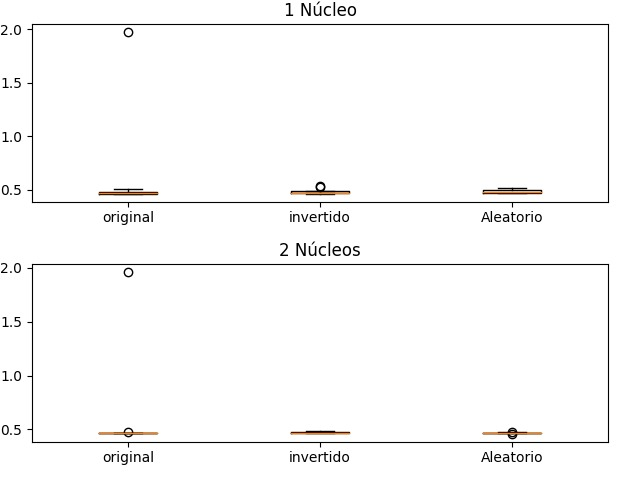
\includegraphics[width=\linewidth]{tareatresparadosmil.jpeg}
           \caption{Gr\'afica para dos mil n\'umeros usando dos procesadores}
           \label{fig:westminster_aerea}
        \end{subfigure}
        \begin{subfigure}[b]{0.45\linewidth}
           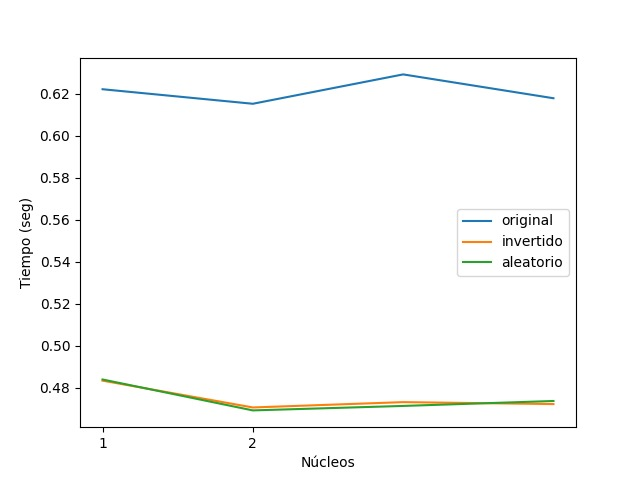
\includegraphics[width=\linewidth]{tareatresparadosmilgrafica.jpeg}
           \caption{Gr\'afica de n\'ucleos contra tiempo.}
           \label{fig:westminster_aerea}
        \end{subfigure}
      \begin{subfigure}[b]{0.45\linewidth}
           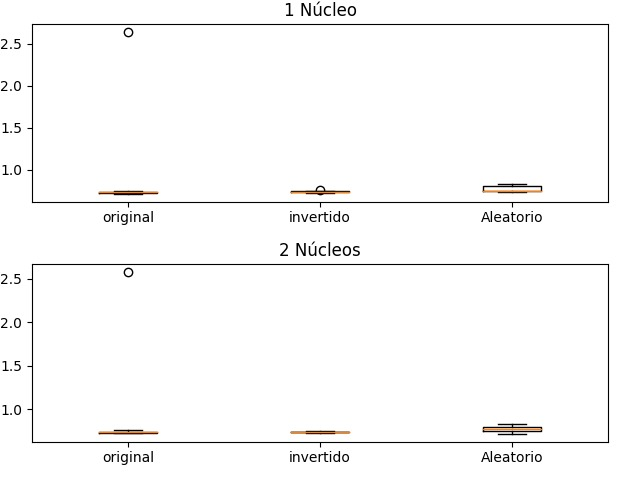
\includegraphics[width=\linewidth]{tareatresparatresmil.jpeg}
           \caption{Gr\'afica para tres mil n\'umeros usando dos procesadores}
           \label{fig:westminster_aerea}
        \end{subfigure}
\begin{subfigure}[b]{0.45\linewidth}
           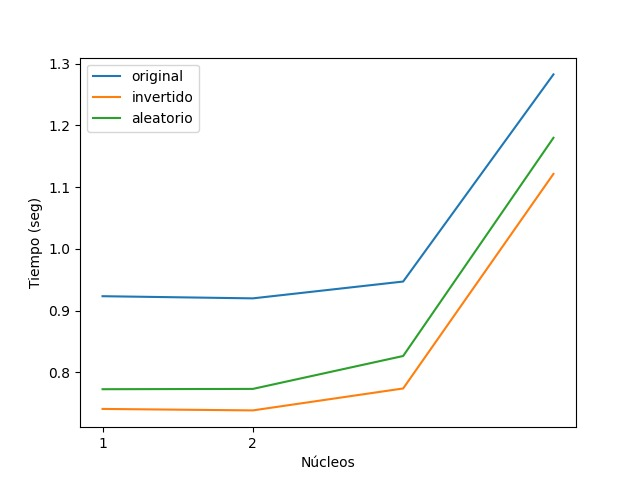
\includegraphics[width=\linewidth]{tareatresparatresmilgrafica.jpeg}
           \caption{Gr\'afica de n\'ucleos contra tiempo}
           \label{fig:westminster_aerea}
        \end{subfigure}
\begin{subfigure}[b]{0.45\linewidth}
           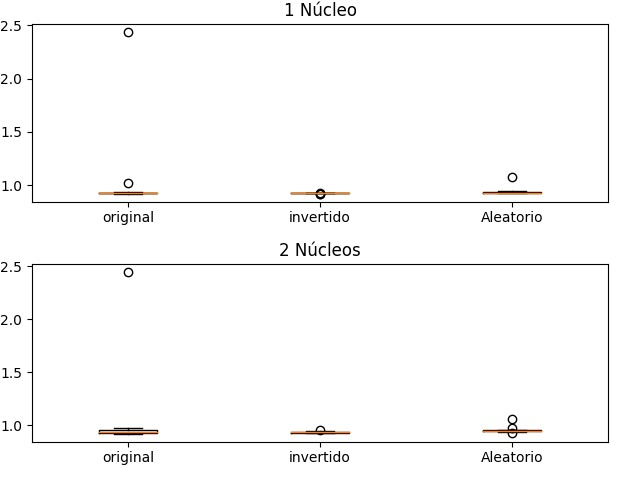
\includegraphics[width=\linewidth]{tareatresparacuatromil.jpeg}
           \caption{Gr\'afica para cuatro mil n\'umeros usando dos procesadores}
           \label{fig:westminster_aerea}
        \end{subfigure}
\begin{subfigure}[b]{0.45\linewidth}
           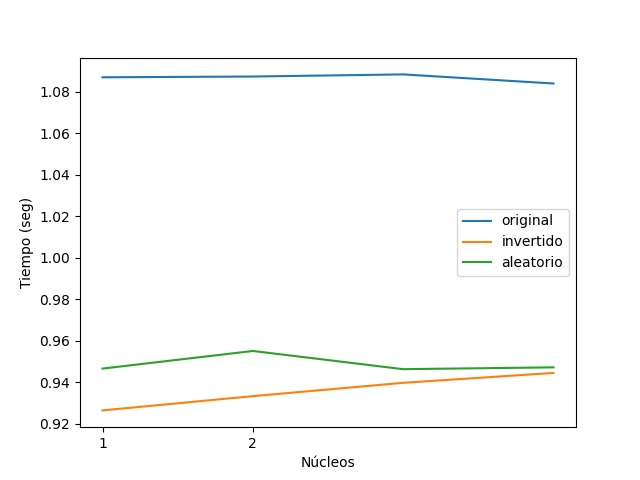
\includegraphics[width=\linewidth]{tareatresparacuatromilgrafica.jpeg}
           \caption{Gr\'afica de n\'ucleos contra tiempo}
           \label{fig:westminster_aerea}
        \end{subfigure}
        \caption{Magnitudes del vector}
        \label{fig:westminster}
\end{figure}

\section{Conclusi\'on}

La simulaci\'on de la ``Teor\'ia de colas'' usando n\'umeros primos usando 8 d\'igitos nos ayud\'o a variar el uso de los n\'ucleos en el procesador y con ello, la diferencia del tiempo que se pude ver en las gr\'aficas.
En el repositorio\citep{yo} se puede encontrar las gr\'aficas y las caracter\'isticas del procesador.

\bibliography{tareatres1}
 \bibliographystyle{plainnat}

\end{document}